En la sexta clase del curso, continuamos trabajando con algor\'itmos de clasificaci\'on de im\'agenes, centrandonoces ne este caso en los no supervisados. Son nuestros objetivos:

\begin{itemize}
  \item Poder realizar clasificaciones no supervisadas utilizando los distintos algoritmos que se encuentran en R.
  \item Calcular la distancia espectral entre como forma de determinar la separabilidad de dos clases espectrales.
  \item Comparar utilizando la entropia de un pixel que coberturas presentan  mayor confusion al momento de la clasificacion.
\end{itemize}

Cargaremos primero la imagen landsat 8 y habilitaremos la opcion para escribir el header de ENVI\@. Usaremos en primer lugar los paquetes \texttt{raster}, \texttt{rgdal}, \texttt{RStoolbox} y \texttt{rasterVis}. Ademass para las clasificaciones vamos a usar las librerias \texttt{e1071}

\begin{lstlisting}
    rasterOptions(addheader = "ENVI")
    xml.2016 <- readMeta("raster_data/LC82240782016304/LC82240782016304LGN00.xml")
    ref.2016 <- stackMeta(xml.2016, quantity = "sre")
    scaleF <- getMeta(ref.2016,xml.2016, what = "SCALE_FACTOR")
    ref.2016 <- ref.2016 * scaleF
    ref.2016 <- ref.2016[[-1,]]
    names(ref.2016) <- c("blue","green","red","nir","swir1","swir2")
    vector <- readOGR(dsn="vector_data", layer="entrenamiento")
\end{lstlisting}

\section{Clasificador por m\'axima verosimilitud}

Empecemos con la clasificacion por el metodo de maxima verosimilitud, para esto necesitamos del paquete

\begin{lstlisting}
    colores = c('#b2df8a','#33a02c',
                '#fdbf6f','#ff7f00',
                '#fb9a99','#e31a1c',
                '#a6cee3','#1f78b4')
    sup.2016 <- superClass(ref.2016, vector, responseCol = "MC_ID",
                           model = "mlc")
    plot(sup.2016$map, col=colores, zlim=c(1,8))
\end{lstlisting}

\begin{figure}
  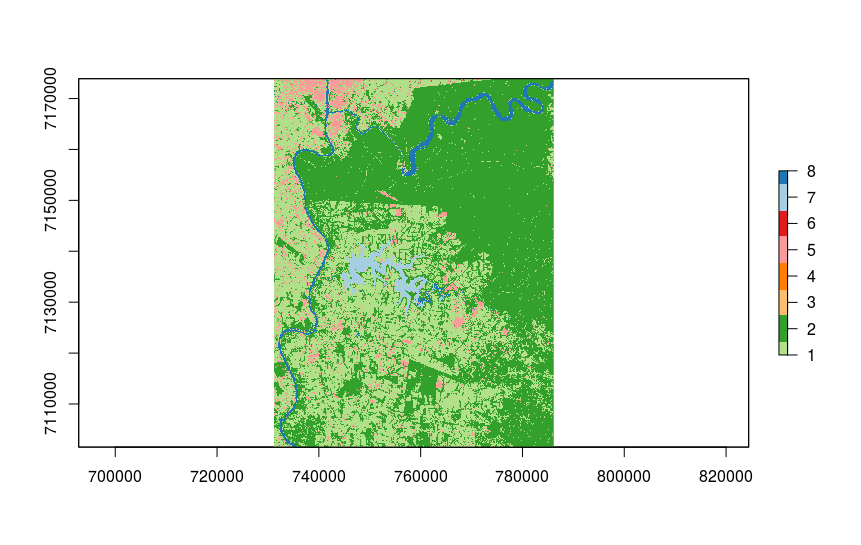
\includegraphics{mlc-MC.png}
  \caption{Clasificacion por maxima verosimilitud sin separar en clases espectrales.}
  \label{fig:MC}
\end{figure}

Cambiando el algoritmo de clasificacion en el parametro \texttt{model} podemoscalcular distintas clasificaciones supervisadas. Algunas de las vistas en clase son \texttt{mlc}, \texttt{rf} y \texttt{svmRadial}. Cada una de ellas usa alguna libreria adicional de las cargadas antes.

\begin{exa}
  Una forma de mejorar las clasificaciones supervisadas basadas en el espacio espectral es clasificar por separado distintas clases espectrales y luego unirlas en la misma clase de informacion. Veams como hacerlo.

  \begin{lstlisting}
      sup.2016b <- superClass(ref.2016, vector, responseCol = "C_ID",
                             model = "mlc")
  \end{lstlisting}

  En este caso, la columna de respuestaa es \texttt{C\_ID} y no \texttt{MC\_ID}.  Una vez realizada la clasificacion, debemos substituir los valores de cada pixel por el de la clase de informacion correspondiente. Para ello hacemos

  \begin{lstlisting}
    subs.2016 = vector@data[c(3,1)]
    sub.2016 <- reclassify(sup.2016b$map, subs.2016)
    writeRaster(sub.2016, "raster_data/processed/mlc2016",
                datatype="INT1U")
  \end{lstlisting}

    Podemos finalmente comparar las dos imagenes clasificadas lado a lado ejecuntado el comando \verb|plot(stack(sup.2016$map,sub.2016),col=colores,zlim=c(1,8))|
    \begin{figure}
      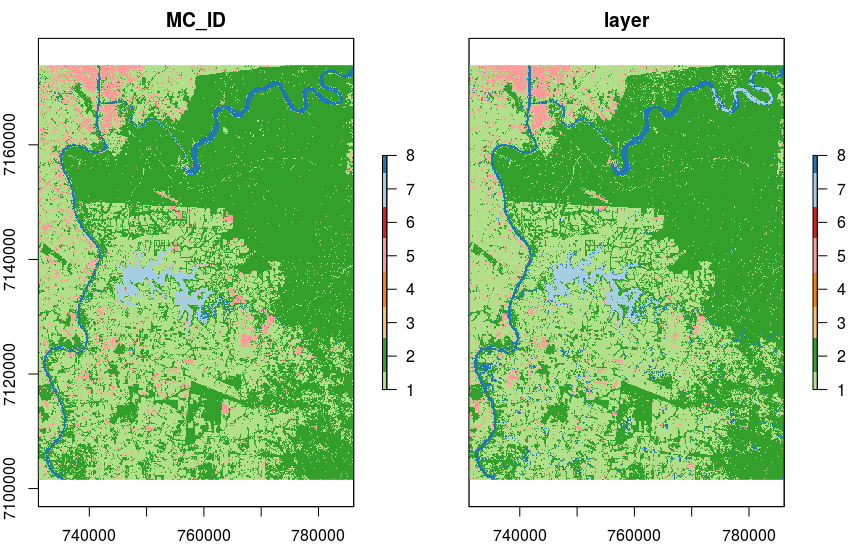
\includegraphics{mlc-comparacion.png}
      \caption{Comparacion entre la clasificacion utilizando clases de informacion y clases espectrales.}
      \label{fig:mlc}
    \end{figure}
\end{exa}

\begin{act}
    Realice clasificaciones por los distintos metodos y comparelas visualmente.
\end{act}

\begin{act}
    Agregue las bandas de textura y evolucion temporal del NDVI y vuelva a clasificar las imagenes.
\end{act}

\section{Entropia de la clasificacion}

Para poder comparar en que zonas los clasificadores presentan mas o menos dispersion podemos calcular la entropia de las distintas clasificaciones en cada pixel. Para esto utilizaremos la funcion \texttt{rasterEntropy}.

\begin{exa}
  Para esto comenzamos corriendo la clasificacion para distintos modelos, los apilados y
  despues calculamos la entropia de los mismos

  \begin{lstlisting}
      set.seed(42)
      library(e1071)
      sup.2016 <- superClass(ref.2016, vector, responseCol = "C_ID",
                           model = "mlc")
      mlc.2016 <- reclassify(sup.2016$map, subs.2016)

      library(randomForest)
      sup.2016 <- superClass(ref.2016, vector, responseCol = "C_ID",
                           model = "rf")
      rf.2016 <- reclassify(sup.2016$map, subs.2016)

      library(kernlab)
      sup.2016 <- superClass(ref.2016, vector, responseCol = "C_ID",
                           model = "svmLinear")
      svm.2016 <- reclassify(sup.2016$map, subs.2016)

      prediction_stack <- stack(mlc.2016, rf.2016, svm.2016)
      names(prediction_stack) <- c("mlc","rf","svm")
      model_entropy <- rasterEntropy(prediction_stack)
  \end{lstlisting}

  Podemos graficar la entropia de las clasificaciones como \verb|model_entropy| y ver que zonas presentan mas diferencias a la hora de la clasificacion y cuales no.
  \begin{lstlisting}
    plot(stack(prediction_stack, model_entropy),col=colores)
  \end{lstlisting}
\end{exa}
  \begin{figure}
    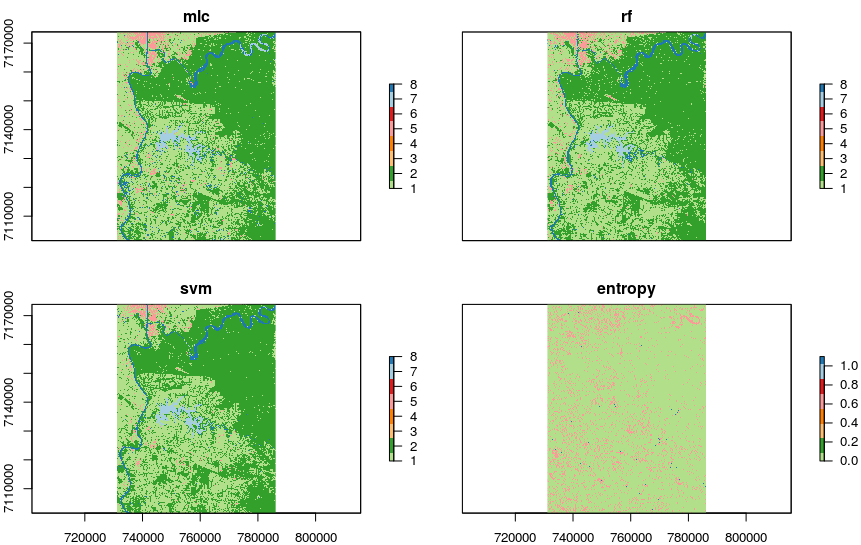
\includegraphics{comparacion-sup.png}
    \caption{Comparacion entre los distintos metodos de clasificacion supervisada usando la entropia de la clasificacion.}
    \label{fig:entropia}
  \end{figure}
\begin{act}
  Repita las clasificaciones por los metodos de arriba agregando la banda textura. Apilela junto con las clasificaciones por k-means de la clase anterior. ¿A que cobertura pertenecen las zonas con mayor variabilidad?
\end{act}
